

\chapter{Étude de la structure d'une archive de courriels en tant que flot de liens}
\minitoc

%L'étude de la structure des réseaux est un sujet qui est étudié depuis assez longtemps \REF.
%Ces études ont, dans un premier temps, permis de trouver comment caractériser une structure puis, dans un second temps, de proposer des méthodes de détections de ces structures.

Nous nous intéressons ici à une archive de courriels publiquement disponibles\footnote{\url{https://lists.debian.org/debian-user/}}.
Cette archive contient l'ensemble des courriels échangés par différent utilisateurs pour résoudre un problème survenu lors de l'utilisation de Debian.
Typiquement, une personne ayant un problème lors de l'installation envoie un courriel à la liste afin de demander de l'aide.
Toute personne inscrite sur la liste reçoit ce courriel et peut y répondre ce qui donne lieu à une discussion visible par tous.
Ces discussions ont déjà été étudiées dans le passé~\cite{dorat2007,sowe2006,wang2014} mais cela a été fait en utilisant des méthodes statiques uniquement.

Or, ces données se représentent naturellement sous forme de flot de liens en associant chaque personne à un n\oe ud et chaque courriel entre deux personnes à un lien dans le flot de liens à l'instant où le courriel a été envoyé.
L'avantage de ces données de communications est que nous connaissons la discussion (\emph{thread}) dans laquelle a lieu chaque message.
Une discussion est un ensemble de courriels dont tout les messages répondent à un message précédent de la discussion excepté pour le premier qui a initié la discussion et que nous appelons \emph{racine}.
Ainsi, nous étudions la structure des discussions dans le flot liens représentant les courriels envoyés sur la liste.

Utiliser le formalisme de flot de liens est particulièrement intéressant car cette lite de diffusion existe depuis 1994.
L'aspect temporel des discussions est donc important.



\section{Prétraitement sur le jeu de données}
Bien qu'accessible sur internet, ce jeu de données nécessite un ensemble de traitements avant de pouvoir exploiter les 724985 courriels que contenait l'archive en janvier 2015.
Tout d'abords, les données ne sont pas sous la forme d'un flot de liens avec la structure des conversations.
Les données sont accessibles via le site internet et ne sont pas structurées.
Pour avoir ces informations sous la forme d'un flots de liens, un script d'extraction a été développé \com{URL}.
Lors de l'extraction, 2269 courriels n'ont pas pu être pris en compte car certaines informations étaient manquantes ou mal formées, typiquement à cause de la date ou d'un fuseau horaire non reconnu.

Une fois les informations brutes récupérées, il faut les transformer en un flot de liens cohérent.
Pour chaque message $m$, nous extrayons son auteur $a(m)$, l'instant $t(m)$ auquel le message a été posté\,\footnote{Cet instant est convertit en $timestamp$ en tenant compte des fuseaux horaires.}, le message auquel il réponds $p(m)$ trouvé via le champ \textsc{In-Reply-To}, son destinataire $a(p(m))$ et la discussion $D(m)$ dans laquelle il apparait.
Comme les messages \emph{racines} ne répondent à aucun autre, nous imposons $p(m)=m$.
L'ensemble de liens du flot est donc $\{(t(m),a(m),a(p(m)))\}_m$.
Nous ne prenons pas en compte la direction des liens.

Une fois le flot créé, il est encore nécessaire de vérifier sa cohérence.
Un message peut être filtré pour différentes raisons: le courriel apparait avant le message auquel il est censé répondre, le message auquel il répond n'est pas présent dans l'archive, l'auteur et le destinataire sont la même personne.
Cette dernière condition permet notamment d'éviter la présence de boucles dans le flot.
Cela concerne principalement les \emph{racines}.
Il s'agit de vérifications simple auquel il faut ajouter les vérifications sur la cohérence de la structure des discussions.
Ainsi, une discussion est entièrement retirée du jeu de données s'il manque la \emph{racine}, si un de ses messages a été retiré à l'étape précédente.
Après ces vérifications, environ $7\%$ des discussions sont retirées.
\'A cela, il faut également tenir compte de notre temps d'observation qui est partiel.
En effet, une discussion dont le dernier message a lieu 1 semaine avant la fin de la capture peut ne pas être terminée.
De même, une discussion durant très longtemps n'a qu'une faible probabilité d'être capturée en entier.
Pour corriger ces biais, nous filtrons également les discussions ayant débutées trop récemment ou durant trop longtemps.
La limite pour considérer une discussion trop récente ou trop longue a été fixé à $4$ ans ($1.26\times 10^8 s$) car nous avons constaté qu'uniquement quelques discussions dépassées ce seuil sur la distribution de durées des discussions dans la figure~\ref{fig:dists_discussion}.
Toutes les discussions qui ont débutées moins de 4 ans avant la capture du jeu de données ne sont donc pas prises en comptes.


Une fois tout ces messages filtrés, nous obtenons un flot de liens avec 316 569 liens entre 34 648 personnes pendant presque 19 ans et 116 999 discussions.
Mis à part les 237 664 messages de début de discussion, ce sont 168 482 courriels qui ont été filtrés soit environ $23\%$.
La majorité des courriels filtrés l'ont été car ils appartiennent à une discussions trop récente.

\section{Caractéristiques élémentaires des discussions}

Les caractéristiques les plus élémentaires des discussions sont le nombre de courriels, le nombres de personnes, le nombre de paires de personnes distinctes en interaction directes et leur durée.
Dans la figure~\ref{fig:dists_discussion}, sont présentées les distributions cumulatives inverses de ces quantités et on remarque qu'elles sont toutes hétérogènes.
On remarque que les données filtrées ne diffèrent pas qualitativement des données brutes.

\begin{figure}
\centering
	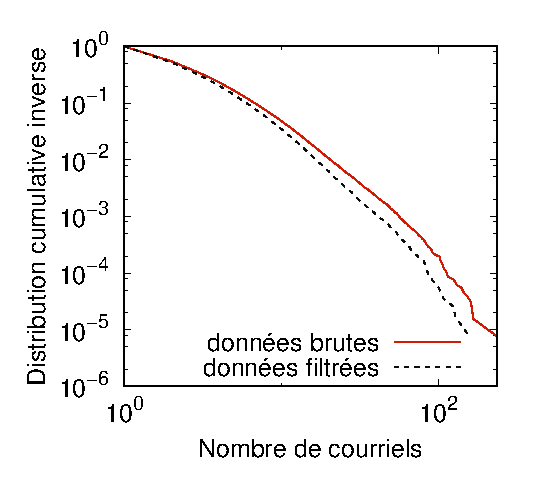
\includegraphics[angle=-90, width=0.49\linewidth]{img/mailing/sizes-ccdf.eps}
	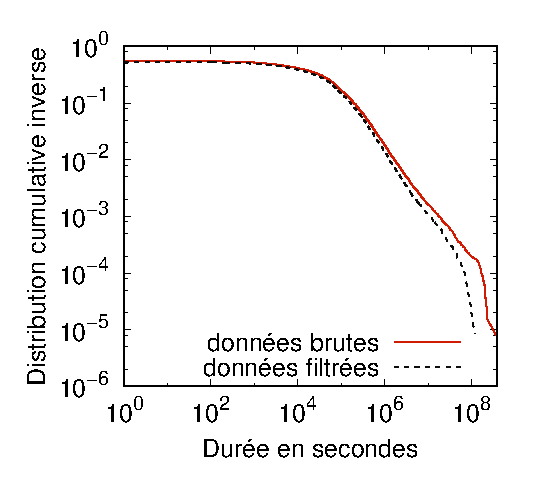
\includegraphics[angle=-90, width=0.49\linewidth]{img/mailing/durations-ccdf.eps}\\
	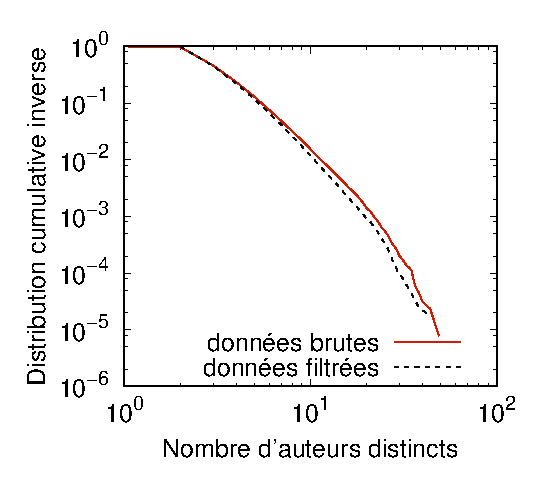
\includegraphics[angle=-90, width=0.49\linewidth]{img/mailing/authors-ccdf.eps}
	\includegraphics[angle=-90, width=0.49\linewidth]{img/mailing/authorpairs-ccdf.eps}
	
	\caption{Distribution cumulative inverse de différentes caractéristiques pour les données brutes (ligne pleine) et filtrées (ligne pointillé). En haut à gauche: nombre de courriels dans une discussion; en haut à droite: durée d'une discussion; en bas à gauche: nombre de personnes dans une discussion; en bas à droite: nombre de paires d'auteurs distinct dans une .}
	\label{fig:dists_discussion}
\end{figure}

La distribution des durées des discussions montre que la majorité des discussions dure environ une journée ou moins ($10^5$ secondes équivaut à moins de 28 heures).
Par ailleurs, on remarque qu'il n'existe que quelques discussions durant plus d'un an.

Ces premières observations sont nécessaires mais pas suffisantes pour comprendre les caractéristiques d'une discussion.
Nous avons également étudié la corrélation entre ces différentes notions et une partie d'entre elles sont présentées dans la figure~\ref{fig:corr_discussion}.


\begin{figure}
	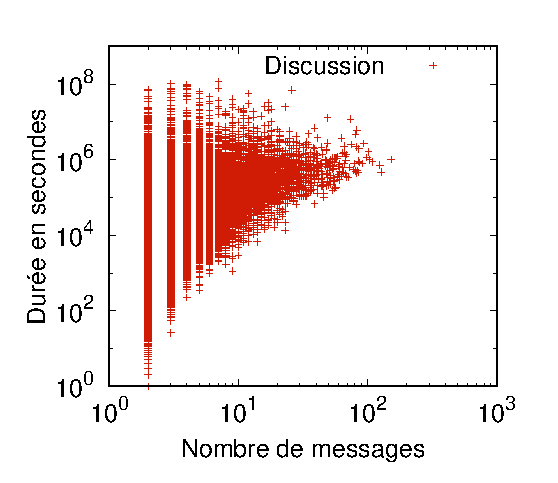
\includegraphics[angle=-90, width=0.49\linewidth]{img/mailing/sizes-durations-corr.eps}
	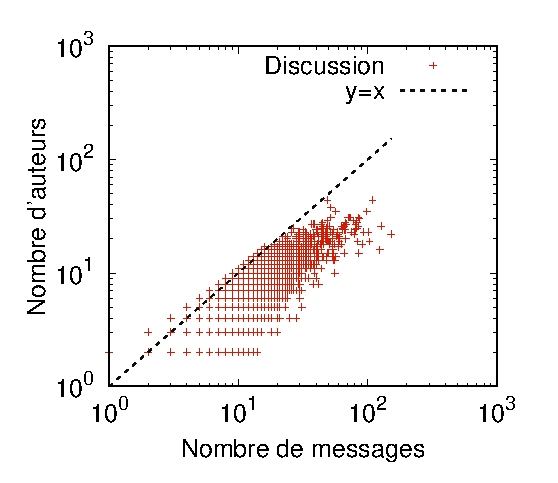
\includegraphics[angle=-90, width=0.49\linewidth]{img/mailing/sizes-authors-corr.eps}
	\caption{Gauche: Corrélations entre le nombre de courriels et la durée d'une discussion. Droite: Corrélation entre le nombre de courriels et le nombre d'auteurs dans une discussion.}
	\label{fig:corr_discussion}
\end{figure}

La corrélation entre la durée et le nombre de courriels, dans la figure~\ref{fig:corr_discussion} partie gauche, met en évidence que plus une discussion est grande en nombre de courriels plus elle dure longtemps, ce qui est attendu.
Par contre, on observe que les petites discussions ont des durées très variables. 
Dans la partie droite de la figure~\ref{fig:corr_discussion} présentant la corrélation entre le nombre de courriels et d'auteurs, on observe un autre fait attendu~\cite{dorat2007} qui est qu'une discussion est constituée, en général, de plus de messages que de participants.
Ainsi lors d'une discussion, c'est un petit nombre de personnes qui échangent potentiellement beaucoup de messages. 

Enfin, il est intéressant d'observer la dynamique des échanges entre deux personnes.
Soit $\tau(u,v) = (t_{i+1}-t_i)_{i=0..k+1}$ la séquence des temps inter-contacts des $k$ liens entre les n\oe uds $u$ et $v$, où $t_0$ est le temps entre $\alpha$ et le premier lien et $t_{k+1}$ est le temps entre le dernier lien et $\omega$.
Il s'agit du temps écoulé avant que deux personnes se contactent à nouveau, indépendamment peu importe la conversation.
Dans la figure~\ref{fig:ict_discussion} est représentée la distribution cumulative inverse du temps inter-contacts. 
$21\%$ des temps inter-contacts sont inférieurs à 30 jours ($2.6\times 10^6 s$).
Ce chiffre bien que relativement faible est tout de même important car il s'agit de discussions ouvertes où tout le monde peut participer. 
En particulier, une personne peut envoyer une demande d'aide à un moment donné et ne plus jamais échanger avec les même personnes.
Or, on observe que $21\%$ des contacts sont renouvelés en moins de 30 jours.
La participation est donc relativement élevée.
\begin{figure}
	\centering
	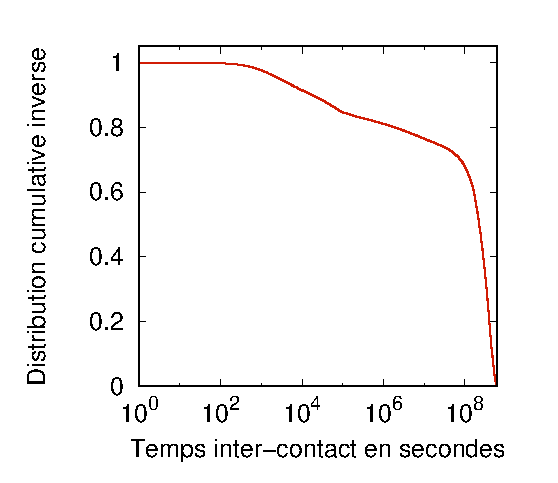
\includegraphics[width=0.49\linewidth]{img/mailing/ict-ccdf.eps}
	\caption{Distribution des temps inter-contacts dans le fil de discussions.}
	\label{fig:ict_discussion}
\end{figure}

\section{\'Etude des discussions en tant que sous-flots}
\label{etude_discussion}
\subsection{Application de la \texorpdfstring{$\Delta$}{delta}-densité}
\label{delta_densite}

Jusqu'à maintenant aucune notion intrinsèquement liée aux flots de liens n'a été utilisée pour caractériser les discussions.
Le but est d'évaluer si cette structure de flot peut se rapprocher d'une structure communautaire.
Comme dit précédemment, les communautés sont souvent définies comme étant des structures devant être densément connectées.
C'est pourquoi nous nous attachons à étudier la densité des discussions.

Comme ces données se modélisent par un flot de liens où les liens n'ont pas de durée, nous étudions la densité non pas dans le flot de liens initial mais dans $\sigma(\xi(\Delta,L))$  pour différentes valeurs de $\Delta$ entre 1 seconde et 20 ans.
La notation $\delta(\sigma(\xi(\Delta,L)))$ est cependant très lourde et nous simplifions par $\delta_{\Delta}(L)$ et nous parlons donc de $\Delta$-densité.
Tout d'abord dans la figure~\ref{fig:dens_fil_discusion} est représentée la $\Delta$-densité globale du le flot.
En couvrant un spectre aussi large de $\Delta$, on observe que la $\Delta$-densité est croissante avec $\Delta$ mais surtout on observe bien la convergence de $\Delta$-densité vers $3.139\times 10^{-4}$, la densité du graphe agrégé, lorsque $\Delta$ est proche de $\omega - \alpha$.

\begin{figure}
	\centering
	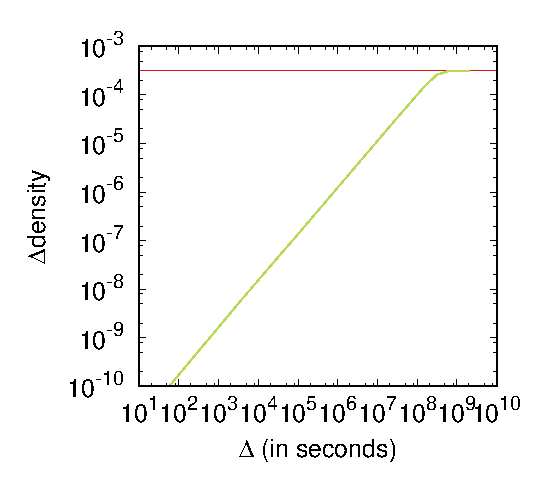
\includegraphics[width=0.48\linewidth]{img/mailing/global_loglog.eps}
	\caption{Évolution de la $\Delta$-densité (en vert) du flot de liens pour $\Delta$ de $60$ seconde à $20$ ans. En rouge, la densité dans le graphe agrégé.}
	\label{fig:dens_fil_discusion}
\end{figure}

Cependant, la $\Delta$-densité du flot n'apporte que peu d'informations en elle-même.
Elle est surtout utile pour comparer les valeurs de $\Delta$-densité des sous-flots que sont les discussions, c'est-à-dire  $\delta(\sigma(\xi(\Delta,D_i)))$.
Ainsi dans la figure~\ref{fig:intra_dens_discussion}, est présentée la distribution cumulative inverse de la $\Delta$-densité des discussions pour différentes valeurs de $\Delta$.
On remarque que les différentes valeurs de $\Delta$ ne semblent pas influencer qualitativement la distribution de $\Delta$-densité.
Cette courbe met surtout en évidence que les discussions sont des structures beaucoup plus denses que le flot.
En effet, la densité médiane des discussions est, selon la valeur de $\Delta$, entre $2.69 \times 10^{-4}$ et $0.28$ alors que le flot a une $\Delta$-densité variant entre $1.05  \times 10^{-10}$ et $3.42 \times 10^{-5}$.
La $\Delta$-densité des discussions est donc en moyenne $10^{5}$ fois plus élevée que celle du flot.
Bien que notable, ce fait est attendu notamment car le flot dure beaucoup plus longtemps et concerne beaucoup plus de n\oe uds que les discussions.
\begin{figure}
\centering
%\subfloat[Inverse cumulative distribution of intra-threads density.]{
	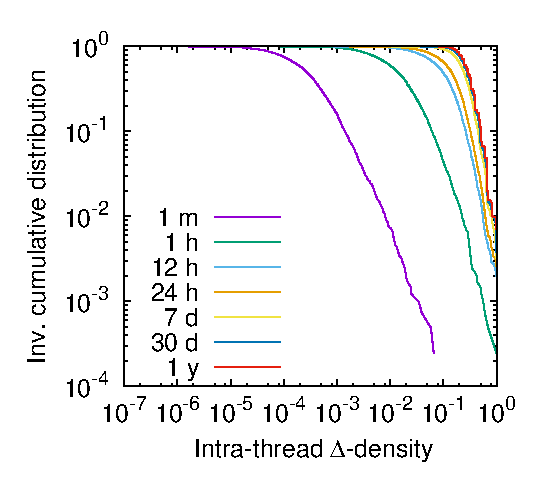
\includegraphics[width=0.48\linewidth]{img/mailing/delta.eps}
%}

\caption{Distribution cumulative inverse de la $\Delta$-densité des discussions pour différentes valeurs de $\Delta$s.}
\label{fig:intra_dens_discussion}
\end{figure}

Afin d'aller plus loin dans l'étude de cette structure, il faut revenir à une définition plus précise de ce qu'est une bonne communauté.
En soit, une valeur de densité n'est pas suffisante pour définir une structure communautaire.
En effet, une discussion ayant une densité de $0.8$ peut  ne pas être une communauté tandis qu'une autre ayant une densité proche de zéro peut être une communauté.
Il faut définir un point de comparaison pour effectivement affirmer qu'une structure est particulièrement dense.
La prise en compte de la densité globale est un début mais n'est pas suffisante.

Une autre définition d'une communauté est qu'elle devrait être plus densément connectée à l'intérieur qu'avec les autres communautés adjacentes.
Pour un graphe $G=(V,E)$ et une communauté $C_i$ de la partition $C = \{C_j\}_{j_1..k}$ de $V$ en $k$ communautés, cela se traduit par le calcul de la densité entre les communautés, $\delta^{inter}(C_i)$ :

\begin{equation}
	\delta^{inter}(C_i) = \frac{1}{|C|-1}\sum_{j, i\ne j}\frac{|\{(u,v)\in E\mbox{ t.q. }u\in C_i\mbox{ and }v\in C_j\}|}{|C_i|\cdot |C_j|}.
\end{equation}
Il s'agit tout simplement de la probabilité qu'un lien existe entre un n\oe ud de $C_i$ et un n\oe ud d'une autre communauté.
Encore une fois, cette notion n'a pas de sens direct dans le formalisme de flot de liens et il est nécessaire de l'adapter.
Pour ce faire, nous définissons la $\Delta$-densité inter discussions entre deux discussions $D_i$ et $D_j$: $\delta^{inter}_{\Delta}(D_i,D_j)$.
Soit $E_{\Delta}= \xi(\Delta,E)$ et $L_{inter}(D_i, D_j) = (T',V',E')$ avec 
$V'= V(D_i \cup D_j)$, $T'=[\beta(D_i \cup D_j), \psi(D_i \cup D_j)]$, et $E' = E_{\Delta} \setminus (D_i \cup D_j)$.
Avec ces définitions, $\delta^{inter}_{\Delta}(D_i,D_j)$ est égale à $\delta^{inter}_{\Delta}(D_i,D_j) = \delta(L_{inter}(D_i, D_j))$.
Il s'agit donc de la densité du flot inter discussions qui est constitué des liens entre les n\oe uds induits par $D_i$ et $D_j$ qui n'appartiennent ni à $D_i$ ni à $D_j$.
Dans la figure~\ref{fig:inter_dens_discussion_ex}, un exemple de flot inter discussion est représenté.

\begin{figure}
\centering
%\subfloat[Inverse cumulative distribution of inter-threads density.]{
	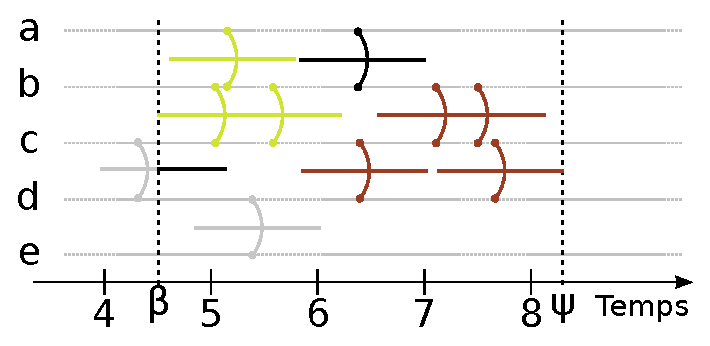
\includegraphics[width=0.8\linewidth]{img/mailing/inter_flot.eps}
%}
\caption{Le flot entre les discussions \textcolor{olivegreen}{\textbf{verte}} et  \textcolor{briquered}{\textbf{rouge}} est constitué des liens ou partie de liens en \textbf{noire}. Les liens en \textcolor{gray}{\textbf{gris}} ne sont pas pris en compte.}
\label{fig:inter_dens_discussion_ex}
\end{figure}



Afin d'obtenir la $\Delta$-densité inter discussions entre $D_i$ et tout les autres discussions, nous utilisons la moyenne des densité inter discussion entre $D_i$ et les autres discussions, soit:

\begin{equation}
	\delta^{inter}_{\Delta}(D_i) = \frac{1}{|C|-1}\sum_{j,i\ne j} \delta^{inter}_{\Delta}(D_i,D_j).
\end{equation}

La distribution cumulative inverse de la $\Delta$-densité inter discussions est présentée dans la figure~\ref{fig:inter_dens_discussion} pour différentes valeurs de $\Delta$.
Bien que similaire, le comportement de la $\Delta$-densité inter discussions diffère qualitativement de celui de la $\Delta$-densité.
La $\Delta$-densité inter discussions croît également en fonction de $\Delta$ mais il y a toujours une différence notable entre $\Delta= 1\  mois$ et $\Delta= 1\ an$ ce qui n'est pas le cas pour la $\Delta$-densité.
Cette différence est normale car lors du calcul de $\Delta$-densité le nombre de liens considérés est fixe peut importe $\Delta$ alors qu'il croît avec $\Delta$ lors du calcul de $\Delta$-densité inter discussions.
Cet effet est visible dans la figure~\ref{fig:inter_dens_discussion_ex}.
Le lien $(c,d)$ qui apparait peut avant $\beta$ n'est pas pris en compte si $\Delta$ est proche de $0$ alors qu'il est en parti pris en compte lorsqu'un $\Delta$ plus grand est considéré, ce qui est le cas dans la figure.

Un autre facteur est aussi la duré considérée qui est plus longue que la durée des discussions.
\begin{figure}
\centering
%\subfloat[Inverse cumulative distribution of inter-threads density.]{
	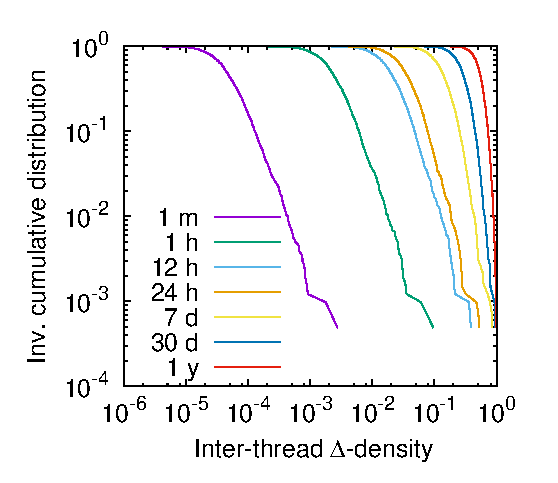
\includegraphics[width=0.48\linewidth]{img/mailing/inter_delta.eps}
%}
\caption{Distribution cumulative inverse de la $\Delta$-densité inter discussions pour différentes valeurs de $\Delta$s.}
\label{fig:inter_dens_discussion}
\end{figure}


Afin de comparer plus aisément $\Delta$-densité et $\Delta$-densité inter discussions, la corrélation entre ces deux mesures est présentée dans la figure~\ref{fig:corel_inter_discussion} pour différentes valeurs de $\Delta$.
On remarque que les discussions sont effectivement plus denses intérieurement qu'avec les autres discussions.
La différence est de plusieurs ordres de grandeur lorsque $\Delta$ est petit et elle diminue lorsque $\Delta$ croît.
Pour $\Delta=20\ ans$ dans la figure~\ref{fig:corel_inter_discussion_20}, la différence n'est plus visible car à cette échelle de temps, l'ancrage temporel des discussions n'est plus décisif.
On remarque tout de même que pour $\Delta=1\ an$, la différence reste notable.
 

\begin{figure}[]
\centering
	\begin{subfigure}{0.48\textwidth}
		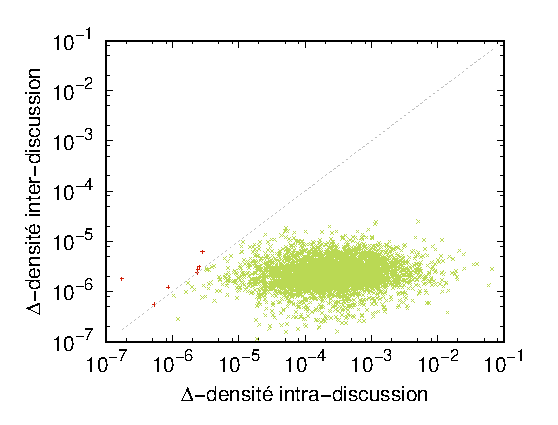
\includegraphics[width=\linewidth]{img/mailing/DensityCurve/120/mean.eps}
		\caption{$\Delta= $1 minute}		
	\end{subfigure}
	\begin{subfigure}{0.48\textwidth}
		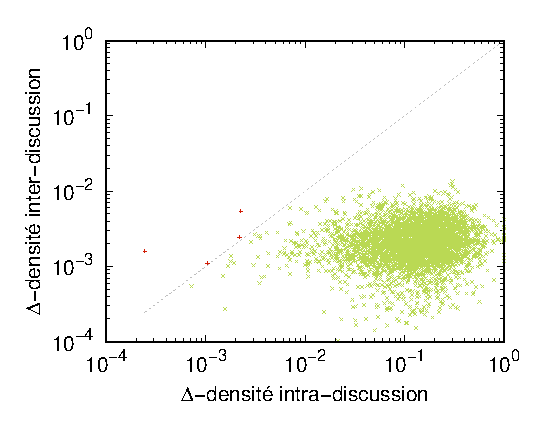
\includegraphics[width=\linewidth]{img/mailing/DensityCurve/172800/mean.eps}
		\caption{$\Delta= $1 jour}		
	\end{subfigure}
	
	\begin{subfigure}{0.48\textwidth}
		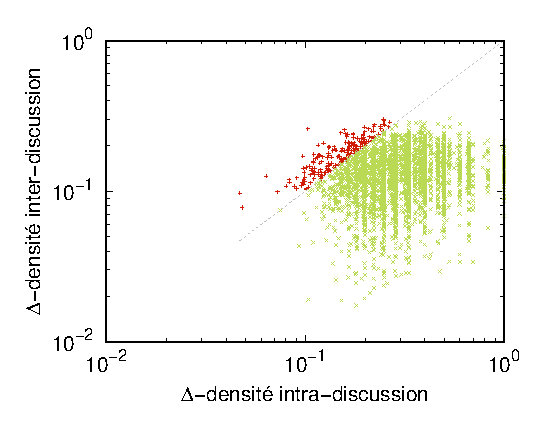
\includegraphics[width=\linewidth]{img/mailing/DensityCurve/63072000/mean.eps}
		\caption{$\Delta= $1 an}		
	\end{subfigure}
	\begin{subfigure}{0.48\textwidth}
		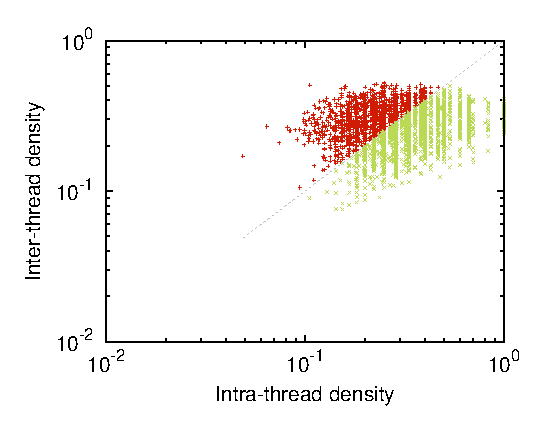
\includegraphics[width=\linewidth]{img/mailing/DensityCurve/1261440000/mean.eps}
		\caption{$\Delta= $20 ans}	
		\label{fig:corel_inter_discussion_20}	
	\end{subfigure}

\caption{Corrélations entre $\Delta$-densité et $\Delta$-densité inter discussions pour différentes valeurs de $\Delta$. Une discussion est en vert (resp. rouge) si elle a une $\Delta$-densité plus (resp. moins) élevée que sa $\Delta$-densité inter discussions.}
\label{fig:corel_inter_discussion}
\end{figure}



\subsection{Répartition temporelle et structurelle des discussions}

Nous avons étudié la densité des discussions et entre les discussions mais il est également intéressant d'observer comment ces discussions sont réparties topologiquement et temporellement.
Pour étudier la répartition des discussions dans le temps, nous construisons un graphe d'intervalle~\cite{Lekkeikerker} $X=(V_X,E_X)$ représentant le chevauchement temporel.
Chaque discussion du flot devient un n\oe ud de $V_X$ et le lien $(i,j)$ existe dans $E_X$ si les discussions $D_i$ et $D_j$ correspondantes ont eu lieu au même instant, \emph{i.e.} $[\alpha_i, \omega_i] \cap [\alpha_j, \omega_j] \neq \emptyset$.
De manière similaire, nous définissons le graphe de chevauchement topologique $Y=(V_Y,E_Y)$.
Les n\oe uds de se graphe représentent encore une fois les discussions du flot et un lien existe entre deux discussions si au moins une personne a participé aux deux, \emph{i.e.} $V(D_i) \cap V(D_j) \neq \emptyset$.

Ces deux graphes sont constitués de 116 999 n\oe uds et d'environ 2 millions de liens pour le graphe de chevauchement temporel et d'environ 63 millions de liens pour le graphe de chevauchement topologique.
Par construction, ces graphes contiennent beaucoup d'informations sur les relations entre les discussions.


Dans la figure~\ref{fig:x-y-graphs_discu}(gauche), est représentée la corrélation entre le degré d'une discussion dans le graphe de chevauchement temporel $X$ et sa durée.
Il y a une corrélation évidente entre ces deux notions lorsque les discussions ont une durée supérieur à $10^5$ secondes.
Plus une discussion dure longtemps, plus elle a de chance d'avoir lieu en même temps que beaucoup d'autres discussions.
On observe également que, même pour les discussions durant moins d'un jour ($8.6 \times 10^4$\,s), il peut y avoir jusqu'à une centaine d'autres discussions actives sur la même période.

\begin{figure}
\centering
	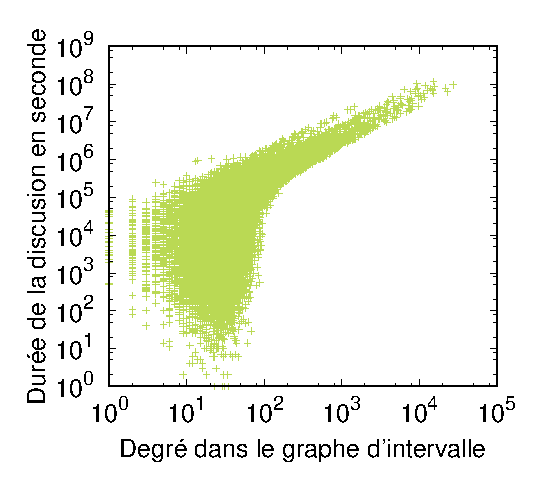
\includegraphics[width=0.49\linewidth]{img/mailing/degree_temp}
	\hfill
	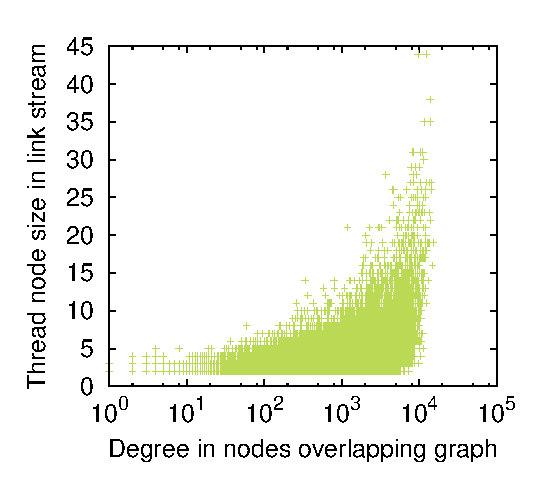
\includegraphics[width=0.49\linewidth]{img/mailing/degree_nodes}
	\caption{Gauche: Corrélation entre le degré des discussions dans le graphe de chevauchement temporel et leur durée. Droite: Corrélation entre le degré des discussions dans le graphe de chevauchement topologique et leur nombre de participants.}
	\label{fig:x-y-graphs_discu}
\end{figure}

La figure~\ref{fig:x-y-graphs_discu}(droite) présente la corrélation entre le degré d'une discussion dans le graphe de chevauchement topologique $Y$ et son nombre de participants.
La corrélation est moins nette mais il y a tout de même une tendance.
Par contre, on remarque de manière frappante que même une petite discussions peut partager des n\oe uds avec les énormément d'autres discussions.


\subsection{Flot quotient}

Le graphe quotient est une autre notion clef pour étudier les relations entre les communautés d'un graphe $G=(V,E)$.
Soit une partition $C= \{C_i\}_{1 .. k}$ des n\oe uds de $G$ en $k$ communautés, chaque communauté est représentée dans le graphe quotient $\bar{G}$ par un n\oe uds dans $V$.
Il y a un lien entre deux communauté $C_i$ et $C_j$ dans $E$ si il existe au moins un lien entre un n\oe uds de $C_i$ et un n\oe uds de $C_j$.
Voir une illustration sur la figure~\ref{fig:graph-quotient}.
Il est possible d'ajouter un poids sur les liens de $\bar{G}$ égale au nombre de liens reliant les communautés.
Le graphe quotient permet de facilement étudier, dans un graphe, les relations entre les communautés.

\begin{figure}
\centering
	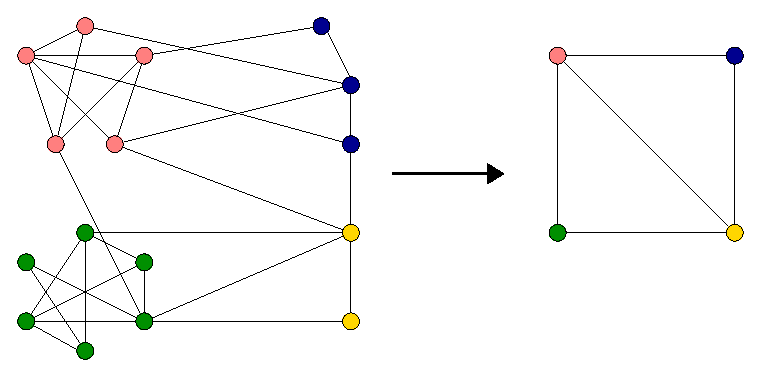
\includegraphics[width=0.50\linewidth]{img/mailing/graph-quotient}
	\vfill
	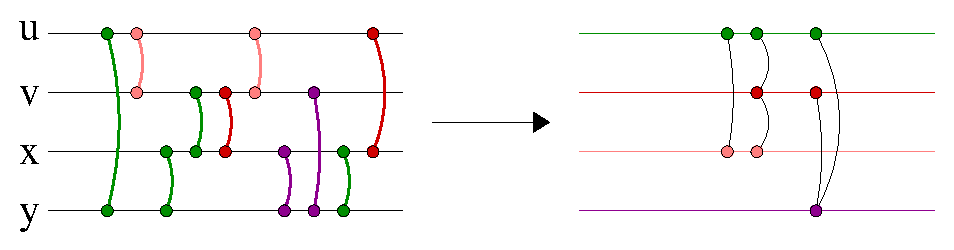
\includegraphics[width=0.75\linewidth]{img/mailing/stream-quotient}
	\caption{Haut: Exemple de graphe ayant une structure communautaire et son graphe quotient associé. Bas: Exemple d'un flot de lien avec une structure ainsi que son flot quotient associé.}
	\label{fig:graph-quotient}
%\label{fig:corel_inter}
\end{figure}

Nous étendons ici cette notion de graphe quotient aux flots de liens.
Nous définissons le flot quotient, $Q=(T_Q,V_Q,E_Q)$, induit par une partition $P=\{{P_i}\}_{1..k}$ en $k$ sous-flots de la manière suivante.
Chaque sous-flot $P_i$ est représenté par un n\oe ud dans $V_Q$.
Il existe un lien $(t,P_i,P_j)$ dans $E_Q$ si il existe $(t_1,u,v) \in P_i$, $(t_2,u,v') \in P_j$ et $(t_3,u,v'') \in P_i$ avec $t_1 \leq t_2 \leq t_3$.
En d'autre termes, il y a un lien dans $E_Q$ si un n\oe ud $u$ a un lien dans $P_j$ qui apparait entre deux autres de ses liens du groupe $P_i$.

Le flot quotient induit par les discussions dans le jeu de données contient 12 281 269 liens impliquant 68 524 discussions différentes.
Comme le jeu de données contient 116 999 discussions, il y a donc 48 475 discussions sans lien et qui ne seront pas prises en compte par la suite.
Ce nombre de discussions non-reliées est élevé comparé à ce qui est obtenu dans un graphe.
En effet dans un graphe, un n\oe ud de degré $0$ correspond à une communauté qui est une composante connexe (ou un union de composantes connexes).
En ajoutant l'information temporelle, les discussions sont séparées par le temps dans flot.
C'est pourquoi un grand nombre de discussions n'ont pas de liens dans le flot quotient.
Ce phénomène est d'autant plus vrai pour les petites discussions.



Il faut aussi noter qu'il y a environ 20 fois plus de liens dans le flot quotient que dans le flot initial.
Cela est normal car un lien dans le flot peut donner lieu à plusieurs liens dans le flot quotient.
Ce cas est visible dans la figure~\ref{fig:graph-quotient}. 
Le lien $(x,y)$ du groupe violet du flot à gauche donne lieu au lien $(\textcolor{plum}{violet}, \textcolor{red}{rouge})$ et au lien $(\textcolor{plum}{violet}, \textcolor{oliveGreen}{vert})$ dans le flot quotient à droite. 

\begin{figure}
\centering
	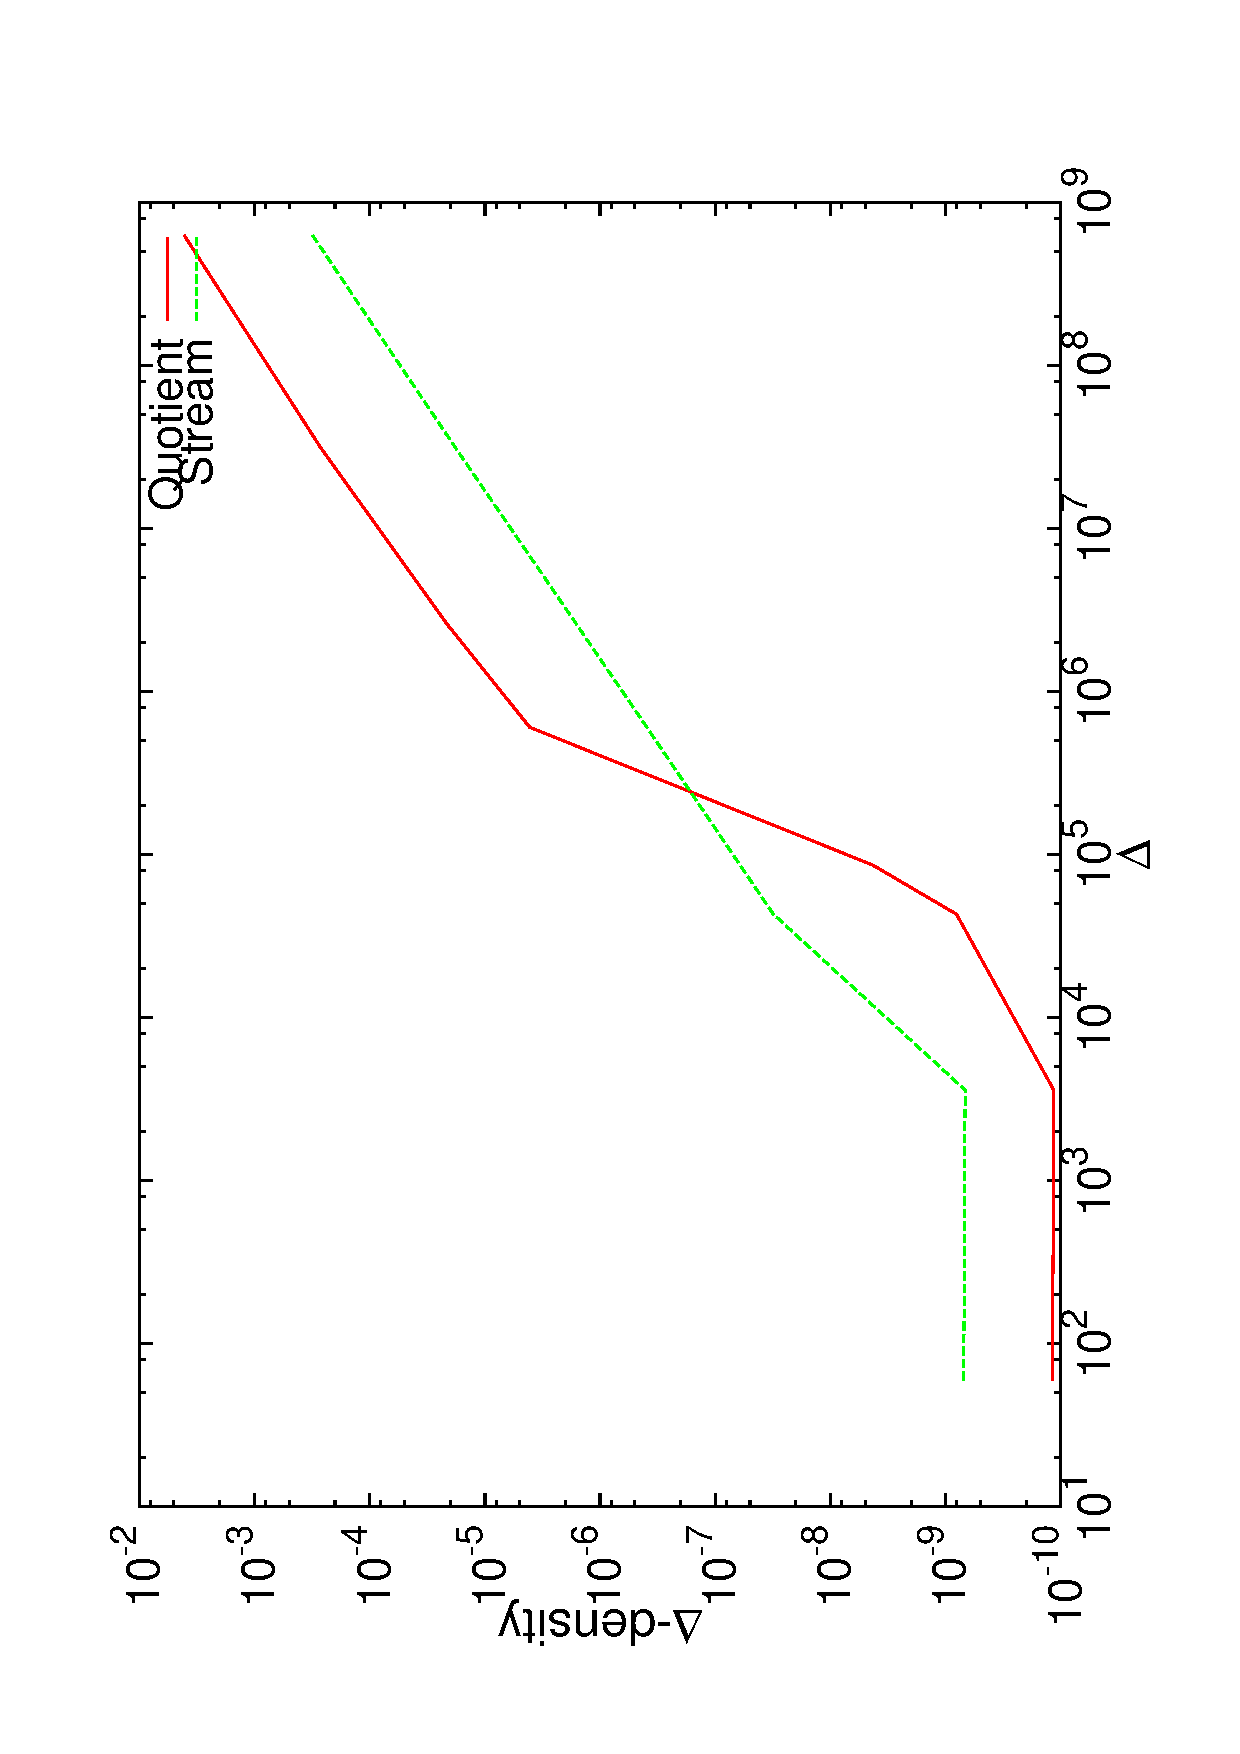
\includegraphics[width=0.71\linewidth]{img/mailing/quotient-density}
	\caption{$\Delta$-densité du flot de liens et du flot de liens quotien en fonction de $\Delta$ pour $\Delta=1mn, 1h, 12h, 1j, 7j, 30j, 1\ an$ et $20\ ans$.}
	\label{fig:quotient-stream-density}
\end{figure}

La figure~\ref{fig:quotient-stream-density} présente la $\Delta$-densité du flot de liens initial et du flot quotient pour différentes valeurs de $\Delta$.
Le flot initial et le flot quotient ont le même comportant de densité mais le flot quotient est moins $\Delta$-dense que le flot initial.
Ce résultat diffère par rapport à ce qui est obtenu dans un graphe.
Cela est dù au nombre de n\oe uds qui augmente dans le flot quotient.
Mais le flot quotient contient tout de même beaucoup de liens. 
En effet, le degré moyen dans le flot quotient est moyenne 25 fois plus élevé que dans le flot.

\subsection{Conclusion}

Nous avons utilisé le modèle de flot de liens pour étudier une archive de courriels provenant du projet Debian.
Grâce au modèle de flot de liens, nous avons étudié des notions clefs pour mieux comprendre la répartition temporelle et topologique des discussions.
Nous avons étudié la notion de $\Delta$-densité sur les discussions en elles mêmes.
Puis, nous avons étudié les relations entre les discussions avec la $\Delta$-densité inter discussions, les projections en graphe de chevauchement temporel ou topologique et le flot quotient.

Cette étude repose en grande partie sur la notion de $\Delta$-densité qui nécessite un paramètre fixé arbitrairement.
Nous avons à chaque fois testé un ensemble de valeurs de $\Delta$ variant d'une seconde jusque parfois 20 ans et, lors de ces tests, aucune valeurs $\Delta$ caractéristique n'a pu être identifiée.
Il semble donc que la $\Delta$-densité soit relativement robuste vis-à-vis de $\Delta$ dans ce contexte.

Nous avons tout d'abord observé que les discussions forment une structure plus dense que le flot de liens.
De manière encore plus forte, nous avons constaté, grâce à la  $\Delta$-densité inter discussion, que les discussions sont plus denses en interne qu'en externe.
C'est une caractéristique importante des communautés que l'on trouve dans les graphes mais qui n'avait pas été observée dans un contexte temporel.
\`A partir de ces observations, nous avons également observé les relations entre les discussions.
Via le graphe de chevauchement temporel, nous avons validé le fait que différentes discussions ont lieu en même temps et que par conséquent une agrégation temporelle entrainerait une perte d'information.
De même via le graphe de chevauchement topologique, on remarque que la structure est très recouvrante sur les n\oe uds, rendant ainsi l'utilisation de partitions statiques de n\oe uds difficilement envisageable pour décrire les discussions.


\section{Détection de structures denses}

\`A partir du constat que les discussions forment une structure particulière, il est naturel d'essayer de les retrouver automatiquement. 
Pour y parvenir, il faut un moyen capable de trouver des sous-flots-denses dans le flots.
C'est à dire une méthode capturant des groupes de liens qui soient proche temporellement et topologiquement.
Il serait tentant d'optimiser directement la densité dans le flot mais ce n'est pas envisageable car un groupe constitué d'un unique lien a une densité de $1$.
Il faut donc trouver une autre méthode.
C'est pourquoi nous avons construit une autre projection du flot en un graphe statique afin d'y appliquer une méthode de détection de communautés.
Le problème est alors de réussir à créer une transformation de telle sorte que les informations temporelles et topologiques ne soient pas complètement détruites.

\subsection{Méthode de détection}
Afin de créer une transformation du flot vers un graphe, nous définissons un autre flot de liens, $\mathfrak{L}$, dont les liens ont une durée.
\`A partir de $\mathfrak{L}$, nous créons un graphe non-orienté et non-pondéré $\mathcal{G} = (\mathcal{V},\mathcal{E})$.

Chaque lien du flot est représenté par un n\oe ud.
Deux liens $(b,e,u,v)$ et $(b',e',u',v') \in \mathfrak{L}$ sont connectés dans le graphe s'ils partagent un n\oe ud et si les intervalles s'intersectent, \emph{i.e.} $\{u,v\} \cap \{u',v'\} \neq \emptyset$ et $[b,e]\cap[b',e'] \neq \emptyset$, voir figure~\ref{fig:Transformation}.
Ainsi, un lien dans le graphe représente une connexion structurelle et temporelle entre deux liens du flot de liens.
Les groupes denses dans le graphe représentent donc des groupes de liens connectés temporellement et topologiquement dans le flot.

\begin{figure}
\centering
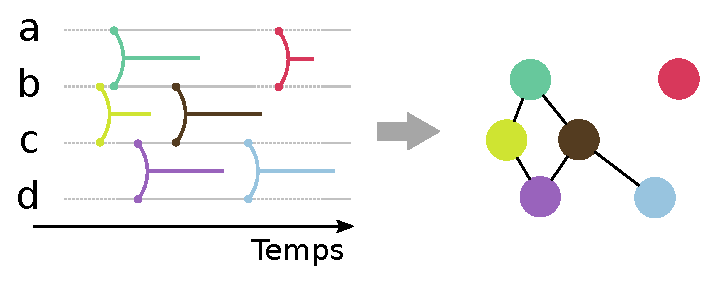
\includegraphics[width=0.6\linewidth]{img/mailing/Transformation.eps}
\caption{Transformation d'un flot de liens avec 4 n\oe uds (a-d) et 6 liens à gauche en un graphe à droite à 6 n\oe uds. La couleur d' un n\oe uds dans le graphe indique le lien du flot qu'il représente.}
\label{fig:Transformation}
\end{figure}%

Il faut donc trouver une manière d'ajouter une durée à chaque lien pour créer $\mathfrak{L}$.
Lors du calcul de la densité dans la section~\ref{delta_densite}, nous avions ajouté une durée arbitraire $\Delta$.
Ici, il n'est pas très pertinent d'appliquer la même logique.
En effet, si on utilise un $\Delta$ faible, alors il n'y aura que très peu de liens dans $\mathcal{E}$ et les n\oe uds représentant les liens d'une discussions ne seront pas forcément connexes.
Il parait illusoire d'espérer retrouver les discussions dans $\mathcal{G}$ si elles ne sont même pas connexes.
Si $\Delta$ est très grand alors toute information temporelle est perdue et cela revient à calculer le line graphe du graphe agrégé.
C'est pourquoi nous adoptons une autre manière d'ajouter une durée sur les liens.

Pour chaque message $m$, nous connaissons $p(m)$, le message auquel il répond dans la discussion.
Nous définissons alors les liens de $\mathfrak{L}$ qui ont une durée de la manière suivante: ${(t(p(m)),t(m),a(m),a(p(m))}_m$.
Ainsi, deux messages, $m_1$ et $m_2$, se succédant dans une discussion sont par définition reliés topologiquement car $a(m_1)= a(p(m_2))$.
Ces deux messages sont aussi reliés temporellement car  nous avons la relation suivante:
\begin{align*}
[t(p(m_1)),t(m_1)]\cap [\mathbf{t(p(m_2))},t(m_2)] &= \\
[t(p(m_1)),t(m_1)]\cap [\mathbf{t(m_1)},t(m_2)] &= [t(m_1)] \neq \emptyset.
\end{align*}
Par construction, une discussion est donc représentée dans $\mathcal{G}$ par un ensemble connexe de n\oe uds.
Un fois $\mathcal{G}$ construit, on peut appliquer un algorithme de détection de communautés.

Avec cette construction, $\mathcal{G}$ contient plus d'1 millions de liens entre 316 569 n\oe uds pour les 116 999 discussions présentes.
Sur ce graphe, nous avons appliqué l'algorithme de Louvain~\cite{Blondel2008a} qui optimise la modularité.
D'autres algorithmes peuvent également être appliqués s'ils capturent des groupes de n\oe uds disjoints et qu'ils passent à l'échelle.
Les groupes trouvés par Louvain sont des communautés dans $\mathcal{G}$.
Par conséquent, ils sont censé être densément connectés dans $\mathcal{G}$.
Comme un lien de $\mathcal{G}$ correspond à une connexion temporelle et topologique dans le flot, on peut espérer qu'ils correspondent à des groupes denses dans le flot.

\subsection{Comparaison des partitions}

Avant de comparer la structure des discussions, $D$, et la partition, $\mathfrak{D}$, trouvée par la méthode de Louvain sur $\mathcal{G}$, il est nécessaire de décrire cette dernière.
Dans la figure~\ref{fig:carac_mail_louvain}, les distributions cumulatives inverses du nombre de liens, du nombre n\oe uds et de leur durée sont présentées pour les groupes de $\mathfrak{D}$.
Pour rappel, les même données sont représentées pour les discussions.
On remarque tout de suite que $\mathfrak{D}$ contient des groupes beaucoup plus gros en nombre de n\oe uds et de liens alors qu'ils ont des durées similaires.
\begin{figure}[]
\centering
	\begin{subfigure}{0.4\textwidth}
		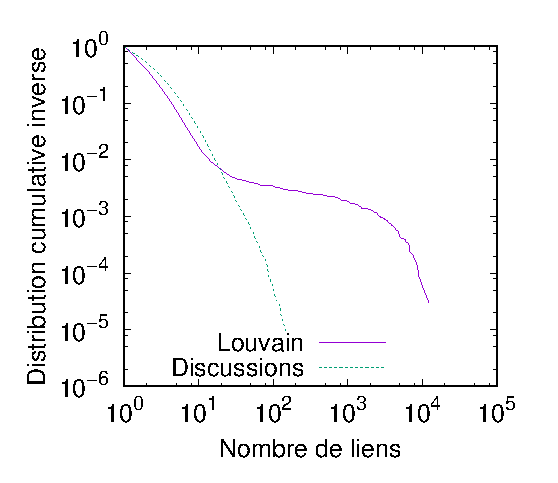
\includegraphics[width=\linewidth]{img/mailing/Detection/linksize}\hfill
		\caption{}		
	\end{subfigure}
	\begin{subfigure}{0.4\textwidth}
		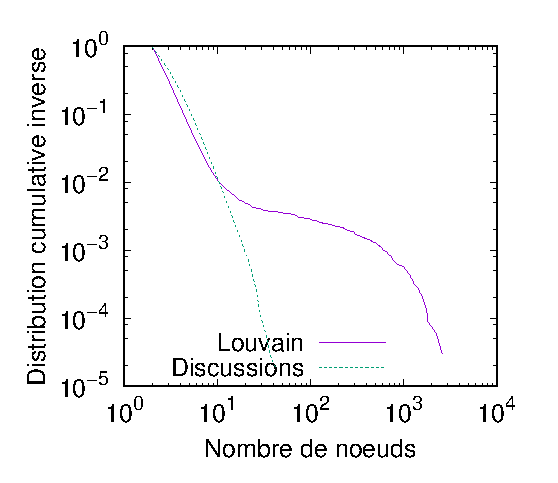
\includegraphics[width=\linewidth]{img/mailing/Detection/nodeSize}\hfill
		\caption{}		
	\end{subfigure}

	\begin{subfigure}{0.4\textwidth}
		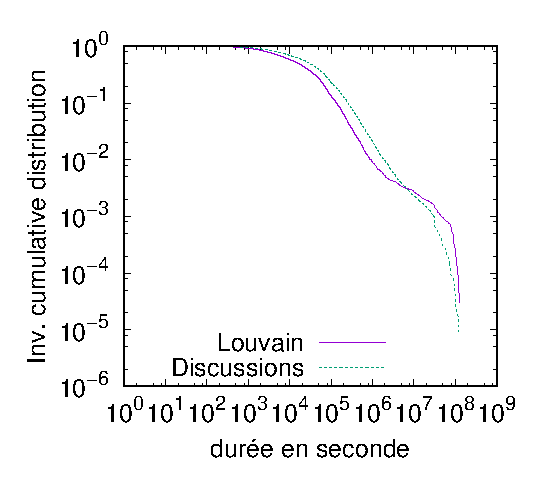
\includegraphics[width=\linewidth]{img/mailing/Detection/duree}\hfill
		\caption{}		
	\end{subfigure}
	\begin{subfigure}{0.4\textwidth}
		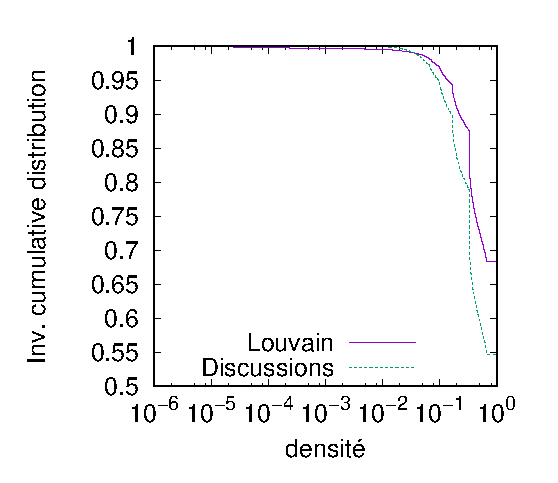
\includegraphics[width=\linewidth]{img/mailing/Detection/densite}
		\caption{\label{fig:dens_mail_louvain}}		
	\end{subfigure}
\caption{Distribution cumulative inverses du nombre de liens (a), du nombre de n\oe uds (b), de la durée (c) et de la densité (d) pour les groupes trouvés par Louvain et les discussions.}
\label{fig:carac_mail_louvain}
\end{figure}



Ces deux structures sont donc très différentes mais cela pourrait être dû à l'algorithme de Louvain qui n'est pas adapté pour trouver des groupes denses.
C'est pourquoi, nous avons également observé la densité des groupes de $D$ et $\mathfrak{D}$ dans le flot $\mathfrak{L}$.
Le résultat est visible dans la figure~\ref{fig:dens_mail_louvain}.
Comme les liens de $\mathfrak{L}$ ont une durée, il est possible d'utiliser directement la densité au lieu de la $\Delta$-densité utilisée précédemment.
On remarque que les groupes de $\mathfrak{D}$, bien que plus gros, sont plus denses que les groupes de $D$.
Cependant la distribution cumulative inverse cache les effets de la taille sur la densité.
Or à nombre de liens égale (entre $2$ et $160$), on remarque que les groupes trouvés par Louvain sont  plus denses en moyenne ,$0.46$ contre $0.38$. 
La médiane est également plus élevée: $0.34$ contre $0.33$.
En revanche, les plus gros groupes ($\mathcal{D}_j|>160$) trouvés par Louvain ont une densité plus faible ce qui peut être dù à leur taille.

Si les groupes de $\mathfrak{D}$ sont plus denses, c'est peut être car ils regroupent plusieurs discussion de $D$ dans un groupe.
Pour comparer deux partitions, l'indice de Jaccard est classiquement utilisé pour calculer la $pr\acute{e}cision$ et le $rappel$ qui sont définis de la manière suivante:

\begin{equation*}
pr\acute{e}cision(\mathfrak{D}_j)= \max_{i} \frac{|\mathfrak{D}_j \cap D_i|}{|\mathfrak{D}_j|}\,, \quad \qquad
rappel(D_i)= \max_{j} \frac{|\mathfrak{D}_j \cap D_i|}{|D_i|}.
\label{eq:rappel}
\end{equation*}

Dans la figure~\ref{fig:rec_inclusion_niveau0}, est présenté la $pr\acute{e}cision$  des groupes et le $rappel$ des discussions en fonctions de leur taille.
Chaque point représente la moyenne du $pr\acute{e}cision$ (resp. $rappel$) pour les groupes (resp. discussions) d'une taille donnée.
On voit qu'il y a un important rappel et ce même pour les grandes discussions, ce qui veut dire qu'en générale une discussion $D_i$ est totalement incluse dans un groupe $\mathfrak{D}_j$.
En revanche, la précision est très faible car un groupe $\mathfrak{D}_j$ contient plusieurs discussions, ce qui est cohérent avec la taille très importante des groupes de $\mathfrak{D}_j$.

\begin{figure}
\centering

\hfill
	\begin{subfigure}{0.49\textwidth}
		\includegraphics[width=\linewidth]{img/mailing/Detection/Rappel_0.eps}
		\caption{}		
	\end{subfigure}\hfill
	\begin{subfigure}{0.49\textwidth}
		\includegraphics[width=\linewidth]{img/mailing/Detection/Precision_0.eps}
		\caption{}		
	\end{subfigure}\hfill

\caption{(A) Rappel des discussions vis-à-vis des groupes trouvés par Louvain.
 (B) Précision des groupes trouvés vis-à-vis des discussions.
Chaque point représente la moyenne du rappel (resp. précision) pour les discussions (resp. groupes) ayant la même taille.
La couleur du point indique le nombre de groupes ayant la même taille.}
\label{fig:rec_inclusion_niveau0}
\end{figure}


Il semble donc que la partition $\mathfrak{D}$ soit proche de $D$ mais que ses groupes soient plus gros.
Pour circonvenir à ce problème, nous appliquons de manière récursive l'algorithme de Louvain sur chaque graphe induit par un groupe $\mathfrak{D}_j$.
Ce processus permet de subdiviser de manière récursive chaque groupe $\mathfrak{D}_j$.
Soit $\mathfrak{D}_{j'}(h)$ un groupe trouvé au niveau $h$, par construction, il est inclus dans un groupe trouvé au niveau $h-1$, c'est à dire $\mathfrak{D}_{j'}(h) \subseteq \mathfrak{D}_{j}(h-1)$.
Le niveau $0$ est la première partition trouvée par l'algorithme de Louvain dans $\mathfrak{G}$.

Soit $D_i \in D$, notons $\mathfrak{D}_{\tilde{j}}(h)$ avec $h \in \mathbf{N}$ le groupe trouvé par la méthode de Louvain au niveau $h$ qui soit le plus proche de $D_i$ au niveau $h$, c'est-à-dire $|\mathfrak{D}_{\tilde{j}}(h)\cap D_i|= \max_{j} |\mathfrak{D}_{j}(h) \cap D_i|$.
Avec ces définitions, on observe la relation suivante: $\mathfrak{D}_{\tilde{j}}(h)\cap D_i \subseteq \mathfrak{D}_{\tilde{j}}(h-1)\cap D_i$.
La définition de $rappel$ de l'équation~\ref{eq:rappel} n'est donc pas adaptée pour les niveaux inférieurs et nous l'adaptons de la manière suivante:

\begin{equation}
rappel(D_i,h)= \max_{j} \frac{|\mathfrak{D}_j(h) \cap D_i|}{|D_i \cap \mathfrak{D}_{\tilde{j}}(h-1)|}.
\end{equation}

Ainsi, le $rappel$ au niveau $h$ prends en compte le maximum d'élément qu'il est possible de trouver à ce niveau.
La définition de $pr\acute{e}cision$ ne pose quant à  elle pas de problème.
La figure~\ref{fig:rec_inclusion} représente le $rappel$ adapté et la $pr\acute{e}cision$ pour le premier et deuxième niveau de récursion de la même manière que pour la figure~\ref{fig:rec_inclusion_niveau0}.
On remarque que, dès le premier niveau, le rappel baisse et que ce phénomène s'amplifie fortement au niveau suivant.
Cela implique que les discussions ne sont plus incluses dans un groupe mais au contraire réparties dans plusieurs.
La précision quant à elle augmente légèrement mais cela est dû à la baisse de la taille des groupes trouvés.
Il semble donc qu'il ne soit pas possible avec cette approche de retrouver automatiquement les discussions.


\begin{figure}
\centering
	\hfill
	\begin{subfigure}{0.49\textwidth}
		\includegraphics[width=\linewidth]{img/mailing/Detection/Rappel_1.eps}
		\caption{niveau 1}		
	\end{subfigure}
	\begin{subfigure}{0.49\textwidth}
		\includegraphics[width=\linewidth]{img/mailing/Detection/Precision_1.eps}
		\caption{niveau 1}		
	\end{subfigure}\hfill
	
	\hfill
	\begin{subfigure}{0.49\textwidth}
		\includegraphics[width=\linewidth]{img/mailing/Detection/Rappel_2.eps}
		\caption{niveau 2}		
	\end{subfigure}
	\begin{subfigure}{0.49\textwidth}
		\includegraphics[width=\linewidth]{img/mailing/Detection/Precision_2.eps}
		\caption{niveau 2}		
	\end{subfigure}\hfill

\caption{(A,B,C) Rappel des discussions vis-à-vis des groupes trouvés par Louvain à différent niveaux récursif.
(B,D,F) Précision des groupes trouvés vis-à-vis des discussions.
Chaque point représente la moyenne du rappel (resp. précision) pour les discussions (resp. groupes) ayant la même taille.
La couleur du point indique le nombre de groupes ayant la même taille.
}
\label{fig:rec_inclusion}
\end{figure}


\subsection{Conclusion}
Nous avons avec cette méthode mis en évidence des groupes denses.
Les groupes trouvés sont plus gros et plus denses que la structure des discussions.
Cependant, ces observations ne remettent pas en cause les conclusions faites dans la section~\ref{etude_discussion} pour plusieurs raisons.
Tout d'abord, les flots de lien étudiés ne sont pas exactement les-mêmes ($L\neq \mathfrak{L}$).
Ce changement de flot est nécessaire pour le fonctionnement de la méthode de détection.
Ensuite, les deux structures ne sont pas complètement différentes car les groupes trouvés semblent en fait agréger plusieurs discussions.
Malheureusement, nous n'avons pas réussi avec notre méthode à isoler chaque discussion malgré notre approche récursive.
Pourtant, il semble que la structure trouvée ai du sens au vu des valeurs de densité des groupes.
